%---------------------导言区---------------------------%
\documentclass[10pt,a4paper,twocolumn,twoside,UTF8]{ctexart}
\usepackage{geometry}
	\geometry{left=2cm,right=2cm,top=2.5cm,bottom=3cm}
\usepackage{xeCJK,amsmath,paralist,enumitem,booktabs,multirow,graphicx,subfig,setspace,listings}
	\setlength{\parindent}{2em}
	\lstset{language=Python}
\usepackage{titlesec}
	\newfontfamily\sectionef{Times New Roman}
	\setCJKfamilyfont{dsf}{Droid Sans Fallback}
 	\newcommand{\sectioncf}{\CJKfamily{dsf}}
  	\titleformat*{\section}{\large\bfseries\sectioncf\sectionef}
    \titleformat*{\subsection}{\normalsize\bfseries\sectioncf\sectionef}
\usepackage{fancyhdr}
\usepackage{layout}
\setlength\columnsep{0.8cm}
%%begin----------设置首页和正文不同的页眉页脚----------------%%
\usepackage{ifthen}
\newboolean{first}
\setboolean{first}{true}
\pagestyle{fancy}
	\fancypagestyle{maincontent}{
		\fancyhf{}  
		\fancyhead[EL, OR]{\thepage}
		\fancyhead[EC]{B2 准稳态法测量不良导体的热导率}
		\fancyhead[OC]{基\quad 础\quad 物\quad 理\quad 实\quad 验}
		\renewcommand\headrulewidth{0pt}
	}
	
	\usepackage{datetime}
	\fancypagestyle{firstpage}{
		\setboolean{first}{false}
		\fancyhf{}  
		\fancyhead[L]{\the\year 年\the\month 月}
		\fancyhead[R]{\shortmonthname[\the\month], \the\year}
		\fancyhead[C]{
		          \large{基\quad 础\quad 物\quad 理\quad 实\quad 验}\\
		          \normalsize{GENERAL PHYSICS LABORATORY}
		          }
	}
	
	\newcommand{\makefirstpageheadrule}{
	\makebox[0pt][s]{\rule[0.6\baselineskip]{\headwidth}{0.3pt}}
	\makebox[0pt][s]{\protect\hspace{-0.34em}\rule[0.75\baselineskip]{\headwidth}{0.3pt}}
	\protect\vspace{-20pt}
	}

	\newcommand{\makeheadrule}{
	\makebox[0pt][l]{\rule[1\baselineskip]{\headwidth}{0.3pt}}
	\protect\vspace{-20pt}
	}

	\renewcommand{\headrule}{
	\ifthenelse{\boolean{first}}{\makeheadrule}
	{\makefirstpageheadrule}
	}
%%end--------------设置首页和正文不同的页眉页脚-----------%%
%%begin-----------------参考文献-----------------------%%

\usepackage[colorlinks,linkcolor=blue,urlcolor=blue,citecolor=blue]{hyperref}
\usepackage[hyperref=true,backend=biber,bibstyle=gb7714-2015,citestyle=numeric-comp,sorting=none,backref=true]{biblatex}
\addbibresource{B2.bib}
%%end-------------------参考文献-----------------------%%

%%%%%%%%%%%%%%%%%%%%%%%%%%%%%%%%%%%%%%%%%%%%%%%%%%%%%%%%%%
%%%%%%%%%%%%%%%%%%%%%%%%%正文开始%%%%%%%%%%%%%%%%%%%%%%%%%%
%%%%%%%%%%%%%%%%%%%%%%%%%%%%%%%%%%%%%%%%%%%%%%%%%%%%%%%%%%

%%begin-------------------中文摘要-----------------------%%
\begin{document}
\title{\LARGE\textbf{B2 准稳态法测量不良导体的热导率} \footnotemark[1]}
\author{\large\textit{黄子维}$^{1}$\footnotemark[2]
\\ \normalsize{(1 \textit{中山大学 中山医学院,广东 广州 }510275)}}
\date{}

\twocolumn[
	\begin{@twocolumnfalse}
	\maketitle  
  	\renewcommand{\abstractname} {} 
	\begin{abstract}
	\vspace{-3em}
	{\bf 摘{} 要:}
	{\small 热传导是三种导热形式之一,热导体导热遵循热传导方程。
    导热系数和比热是描述热导体导热性能的两个重要参量。
    本实验中,我们基于热电偶测温,采用准稳态法测量有机玻璃材料和橡胶材料的导热系数与比热,以探究不良导体的导热规律。
    实验测得有机玻璃材料比热为$1423.5 \pm 2.7 J \cdot kg^{-1} \cdot  ^{\circ}C^{-1}$,导热系数为$\lambda = 0.17166 \pm 0.00033 W \cdot m^{-1} \cdot K^{-1}$;
    橡胶材料比热为$1349.2 \pm 4.1 J \cdot kg^{-1} \cdot  ^{\circ}C^{-1}$,导热系数为$\lambda = 0.38147 \pm 0.00100 W \cdot m^{-1} \cdot K^{-1}$}。
	\par
	\textbf{关键词}:准稳态法,不良导体,热电偶,比热,导热系数
	\vspace{2em}
	\end{abstract}
	\end{@twocolumnfalse}
]
\renewcommand{\thefootnote}{\fnsymbol{footnote}}
\footnotetext[1]{由中山大学物理学院陆佑堂提供器材和指导。}
\footnotetext[2]{通信作者,\url{huangzw29@mail2.sysu.edu.cn}}
%%end-------------------中文摘要-----------------------%%

\thispagestyle{firstpage} %首页风格
\pagestyle{maincontent} %其他页风格

%%begin-------------------引言-----------------------%%
\section{引 \quad 言}
热传导是三种导热形式之一,热导体导热遵循热传导方程。
导热系数和比热是描述热导体导热性能的两个重要参量。
导热系数定义为单位温度梯度下每单位时间内由单位面积传递的热量,单位为 $W/( m \cdot  K )$。
比热定义为单位质量某种物质在温度升高(或降低)$1^{\circ}C$时所吸收(或放出)的热量,单位为 $J /( kg \cdot K )$。
热的不良导体导热系数低,导热慢,可以起到保温作用,在许多领域具有广泛应用。

为测量不良导体的比热和导热系数,实验采用准稳态法进行测量,
该方法只需满足导体两端温差恒定以及导体升温速率恒定即可。
相比稳态法而言,该方法具有条件容易实现,易测量,误差小,可重复性和一致性好的优点。

实验采用铜-铜镍热电偶测量温度。热电偶能将温度转换为测温电路电压,
从而能即时方便读出温度值,具有测量简便,精度高的优点。

本实验中,我们基于热电偶测温,采用准稳态法测量有机玻璃材料和橡胶材料的导热系数与比热,以探究不良导体的导热规律。
\newpage %换栏

%%end-------------------引言-----------------------%%

%%begin-------------------正文-----------------------%%
\section{准稳态法实验原理\autocite{shenJiChuWuLiShiYan2015}}

    
准稳态法原理的依据是热传导方程。实验测量材料为方形板状,可抽象为无限大平板导热模型。

考虑厚度为$2R$,初始温度为$t_0$的一维无限大不良导体平板,如图\ref{fig:illus-1}。
\begin{figure}[htbp]
	\centering
	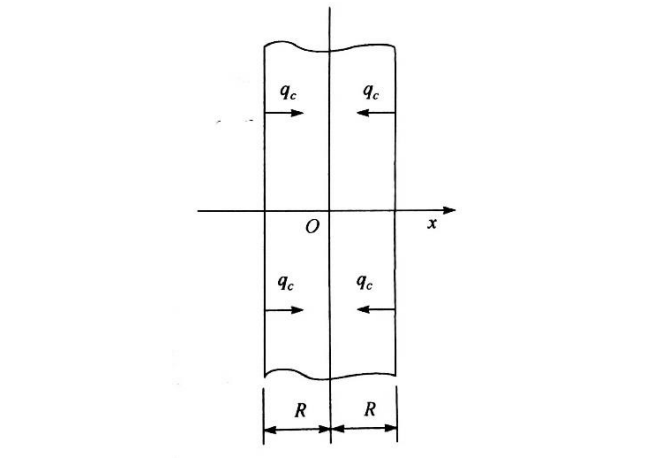
\includegraphics[width=0.4\textwidth]{attachments/illus-1.png}
	\caption{电容电桥}
	\label{fig:illus-1}
\end{figure}

在平板两侧同时施加均匀的指向中心面的热流密度$q_c$,则平板上各处的温度将随加热时间$\tau$变化,
故x处的温度可表示为$t ( x , \tau )$。
以样品中心为坐标原点,则上述模型的热传导方程可写为: 
\begin{equation}
	\left\{
	\begin{aligned}
	&\frac{\partial t ( x , \tau )}{\partial \tau} - \frac{a \partial ^2 t ( x , \tau )}{\partial x^2} = 0\\
	&\frac{\partial t ( R , \tau )}{\partial x}=\frac{q_c}{\lambda}; \frac{\partial t ( 0 , \tau )}{\partial x} = 0\\
	&t(x,0)=t_0
	\end{aligned}
	\right.
	\label{eq:1.1}
\end{equation}

其中$a=\frac{\lambda}{\rho c}$,$q_c=c \rho R\frac{\partial t}{\partial \tau}$。
$\lambda$为材料的导热系数;$\rho$ 为材料密度;c为材料的比热。

当加热时间$\tau$满足$\frac{a\tau}{R^2}>0.5$时,$\tau$的求和项可忽略,方程的解为:
\begin{equation}
	t(x,\tau)=t_0+\frac{q_c}{\lambda}\left(\frac{a}{R}\tau+\frac{1}{2R}x^2-\frac{R}{6}\right)
	\label{eq:1.2}
\end{equation}
故被测样品中心和表面处的温度分别为:
\begin{equation}
	\left\{
	\begin{aligned}
	&t(0,\tau)=t_0+\frac{q_c}{\lambda}\left(\frac{a}{R}\tau-\frac{R}{6}\right)\\
	&t(R,\tau)=t_0+\frac{q_c}{\lambda}\left(\frac{a}{R}\tau+\frac{R}{3}\right)\\
	\end{aligned}
	\right.
	\label{eq:1.3}
\end{equation}
升温速率$v$和加热面与中心面间温度差$\Delta t$为:
\begin{align}
	v &= \frac{a q_c}{\lambda R}  \\
	\Delta t &= \frac{q_cR}{2\lambda} \label{eq:1.4}
\end{align}

可见,该状态下被测样品各处匀速升温,而$\Delta t$与加热时间$\tau$无关,保持恒定,这种状态称为准稳态。
在准稳态条件下,可以求出样品比热$c$和导热系数$\lambda$。
\begin{align}
	c &=\frac{q_c}{\rho R \frac{dt}{d\tau}} \label{eq:1.5.1} \\
	\lambda &= \frac{q_c R}{2\varDelta t} \label{eq:1.5.2}
\end{align}

因此只要在准稳态下测量样品表面和中心处的温度差及样品的升温速率,即可计算样品比热$c$和导热系数$\lambda$。

\section{实验仪器和样品}
	\paragraph{A. 比热/导热系数实验仪(ZKY-BRDR)}~
	\newline 
	\indent
	比热/导热系数实验仪具备为加热器提供电源、测量加热时间以及测量热电偶热电动势的功能,可以方便测量导体比热/导热系数。
	实验仪面板如图\ref{fig:illus-2}所示。
	\begin{figure}[htbp]
        \centering
        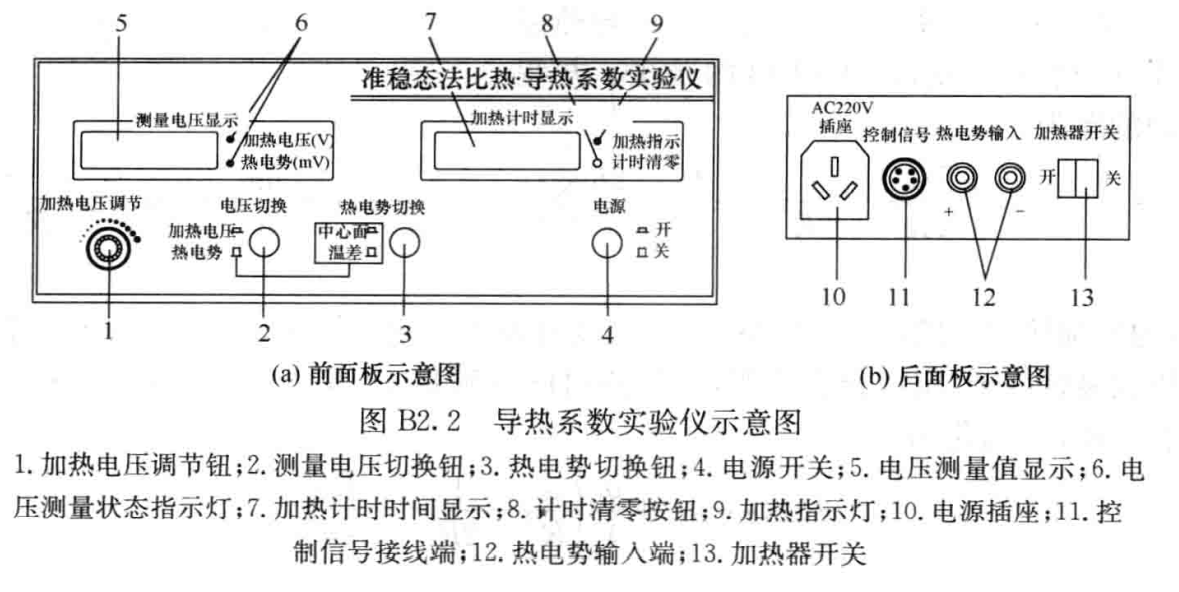
\includegraphics[width=0.4\textwidth]{attachments/illus-2.png}
        \caption{比热/导热系数实验仪}
        \label{fig:illus-2}
    \end{figure}
	
	需注意的是实验仪只有一个电压输入端口,因此需使用测控电路切换待测电压。

	\paragraph{B. 带保温杯的样品架}~
	\newline 
	\indent
	样品架与保温杯如图\ref{fig:illus-3.1}所示。热电偶接线如图\ref{fig:illus-3.2}所示

	\begin{figure}[htbp]
		\centering
		\subfloat[样品架]{\label{fig:illus-3.1}
		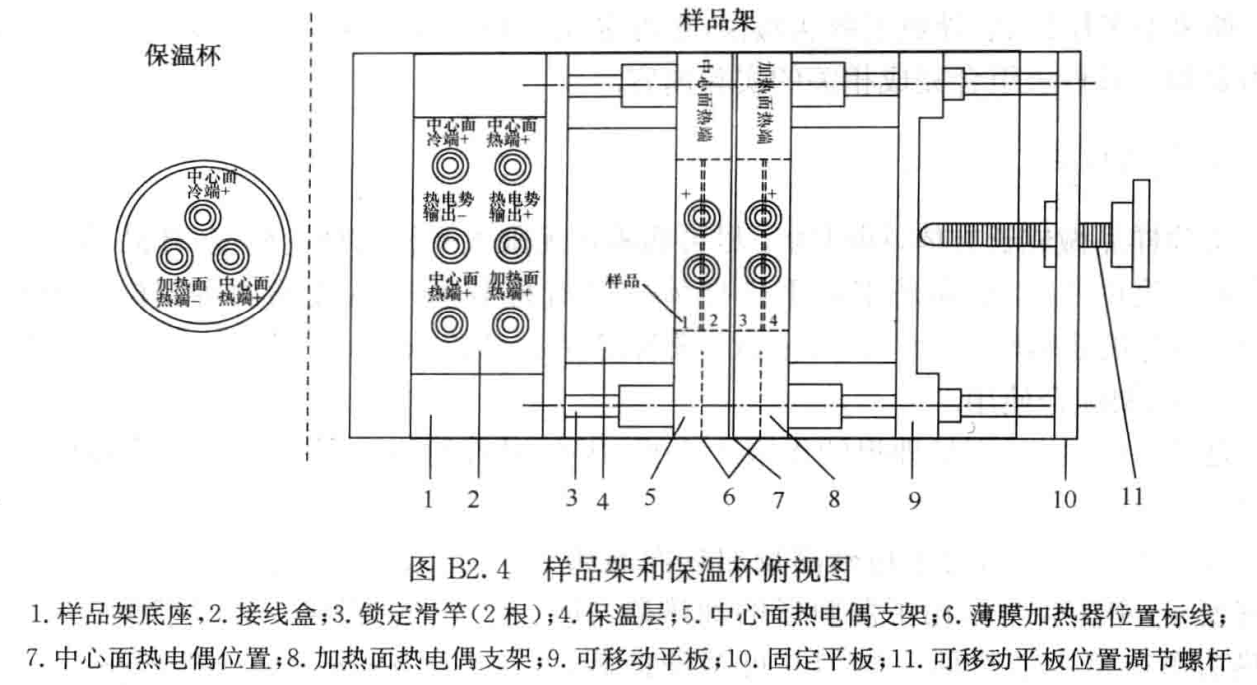
\includegraphics[width=0.23\textwidth]{attachments/illus-3.1.png}
		}	
		\subfloat[热电偶接线]{\label{fig:illus-3.2}
		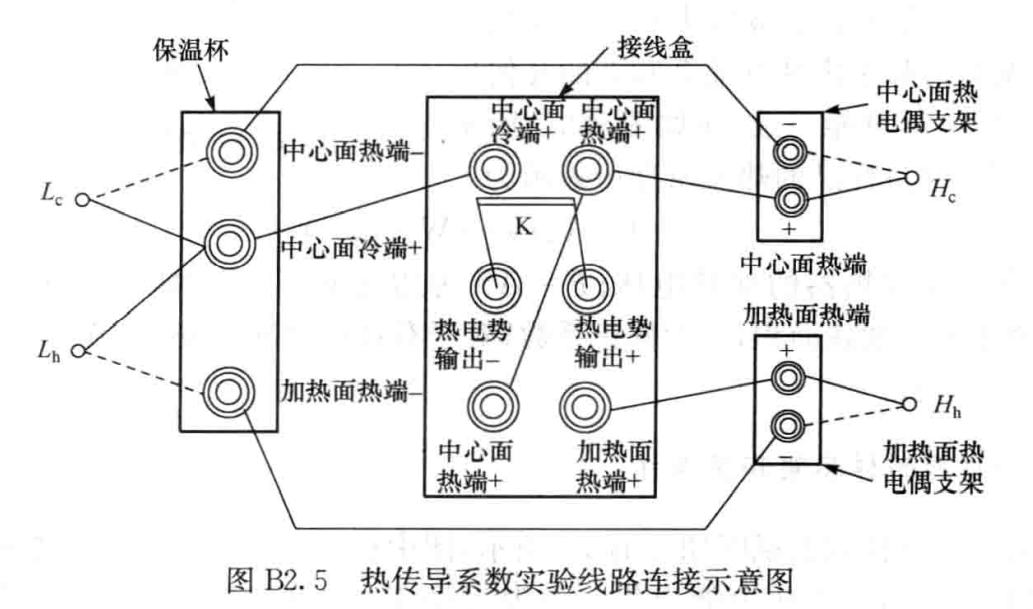
\includegraphics[width=0.23\textwidth]{attachments/illus-3.2.png}
		}
		\caption{样品架和接线}
	\end{figure}

	\begin{enumerate}[label=\arabic*.]
		\item 保温杯:可以提供恒温冷端。实验中将两热电偶冷端接触后放入保温杯中,以保证两热电偶冷端温度相同。
		\item 调节螺钉:旋动螺钉,可以夹紧或松开样品架,以取放样本。
		\item 铜-铜镍热电偶:将温度信号转换为热电势信号,测量温度。
		\item 接线盒:放大热电势信号,以减少信号干扰;内置继电器,可以切换输出中心面热电势$U_C$和温差热电势$\Delta U$。
	\end{enumerate}
	
	\paragraph{C. 待测样品与装置}~
	\newline 
	\indent
	本实验测量样品为有机玻璃(密度$\rho = 1196 kg/m^3$)与橡胶(密度$\rho = 1374 kg/m^3$)。

	为尽可能贴近无限大导热模型,样品形状为正方形薄板。然而,样品并非理想无限大导热模型,因此在计算面积时应引入边缘修正。修正后加热面积$F$为
	\begin{equation}
		F = \frac{S}{A} \label{eq:2}
	\end{equation}
	$S$为实际面积,$A$为修正系数,取为$A=0.85$。

	样品在样品架中的装置如图\ref{fig:illus-4}。
	\begin{figure}[htbp]
        \centering
        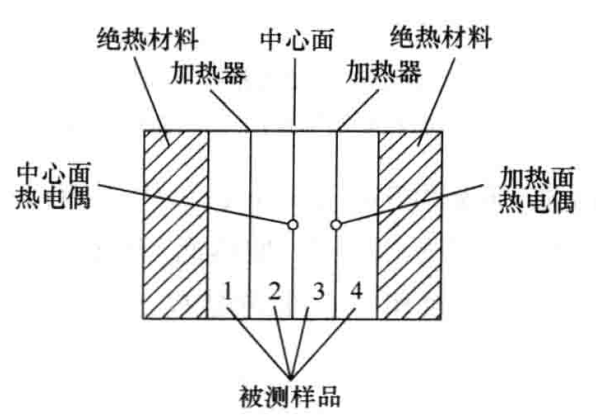
\includegraphics[width=0.3\textwidth]{attachments/illus-4.png}
        \caption{样品在样品架中的装置}
        \label{fig:illus-4}
    \end{figure}
	四块样品两两夹持薄膜加热器,保证样品均匀加热且两侧热阻相同,则热流密度$q_c$为加热功率的一半。
	\begin{equation}
		q_c = \frac{U^2}{2Fr}	\label{eq:3}
	\end{equation}
	$U$为加热电压,$r$为加热器电阻。
	
	两测温热电偶分别在中心面和其中一个加热面。

\section{实验步骤}
	\begin{enumerate}[label=\arabic*.]
		\item 测量样品尺寸
		\item 安装样品:松开调节螺钉,放入充分冷却后的样品,注意\#2和\#3样品厚度应相近。旋进螺钉,压紧样品和热电偶。
		\item 打开主机电源,设定加热电压。本实验加热电压设置为$17.0V$。
		\item 打开加热开关,开始加热。
		\item 测量热电动势:每隔$30s$,记录一次中心面热电势$U_C$和温差热电势$\Delta U$。
		\item 由标定关系计算导热系数$\lambda$和热容$c$。
		\item 更换另一材质样品,按上述步骤测量。
	\end{enumerate}

\section{实验结果}
	\subsection{材料尺寸}
	有机玻璃尺寸如表\ref{tab:1.1},橡胶材料尺寸如表\ref{tab:1.2}。
	\begin{table}[htbp]
    	\centering
    		\begin{tabular}{ccc}
				\toprule
				样品	&宽度$/m$ &厚度$/m$ \\
				\midrule
				A	&0.08967$\pm$0.00007	&0.01005$\pm$0.00003	\\
				B	&0.08964$\pm$0.00002	&0.01011$\pm$0.00002	\\
				C	&0.08964$\pm$0.00001	&0.01002$\pm$0.00002	\\
				D	&0.08962$\pm$0.00003	&0.01003$\pm$0.00003	\\
				\bottomrule
			\end{tabular}
			\caption{\textbf{有机玻璃样品尺寸}}
			\label{tab:1.1}
    \end{table}
			
	\begin{table}[htbp]
    	\centering
    	\begin{tabular}{ccc}
			\toprule
			样品	&宽度$/m$ &厚度$/m$ \\
			\midrule
			A	&0.08943$\pm$0.00022	&0.01004$\pm$0.00002	\\
			B	&0.08938$\pm$0.00007	&0.01006$\pm$0.00002	\\
			C	&0.08970$\pm$0.00005	&0.01023$\pm$0.00002	\\
			D	&0.08927$\pm$0.00021	&0.01007$\pm$0.00001	\\
			\bottomrule
		\end{tabular}
		\caption{\textbf{橡胶样品尺寸}}
		\label{tab:1.2}
    \end{table}

	比较有机玻璃样品样品尺寸:C号和D号样品厚度最为接近,因此置于中心面两侧。计算样品平均厚度和面积:
	\begin{align}
		R &= 0.01003 \pm 0.00002 m \\
		S &= 0.00803 \pm  0.00000 m^2 
	\end{align}

	比较橡胶样品样品尺寸:B号和D号样品厚度最为接近,因此置于中心面两侧。计算样品平均厚度和面积:
	\begin{align}
		R &= 0.01006 \pm 0.00001 m \\
		S &= 0.00798 \pm  0.00002 m^2 
	\end{align}

	\subsection{测量有机玻璃材料导热系数$\lambda$和热容$c$}

	有机玻璃升温曲线如图\ref{fig:1}
	\begin{figure}[htbp]
		\centering
		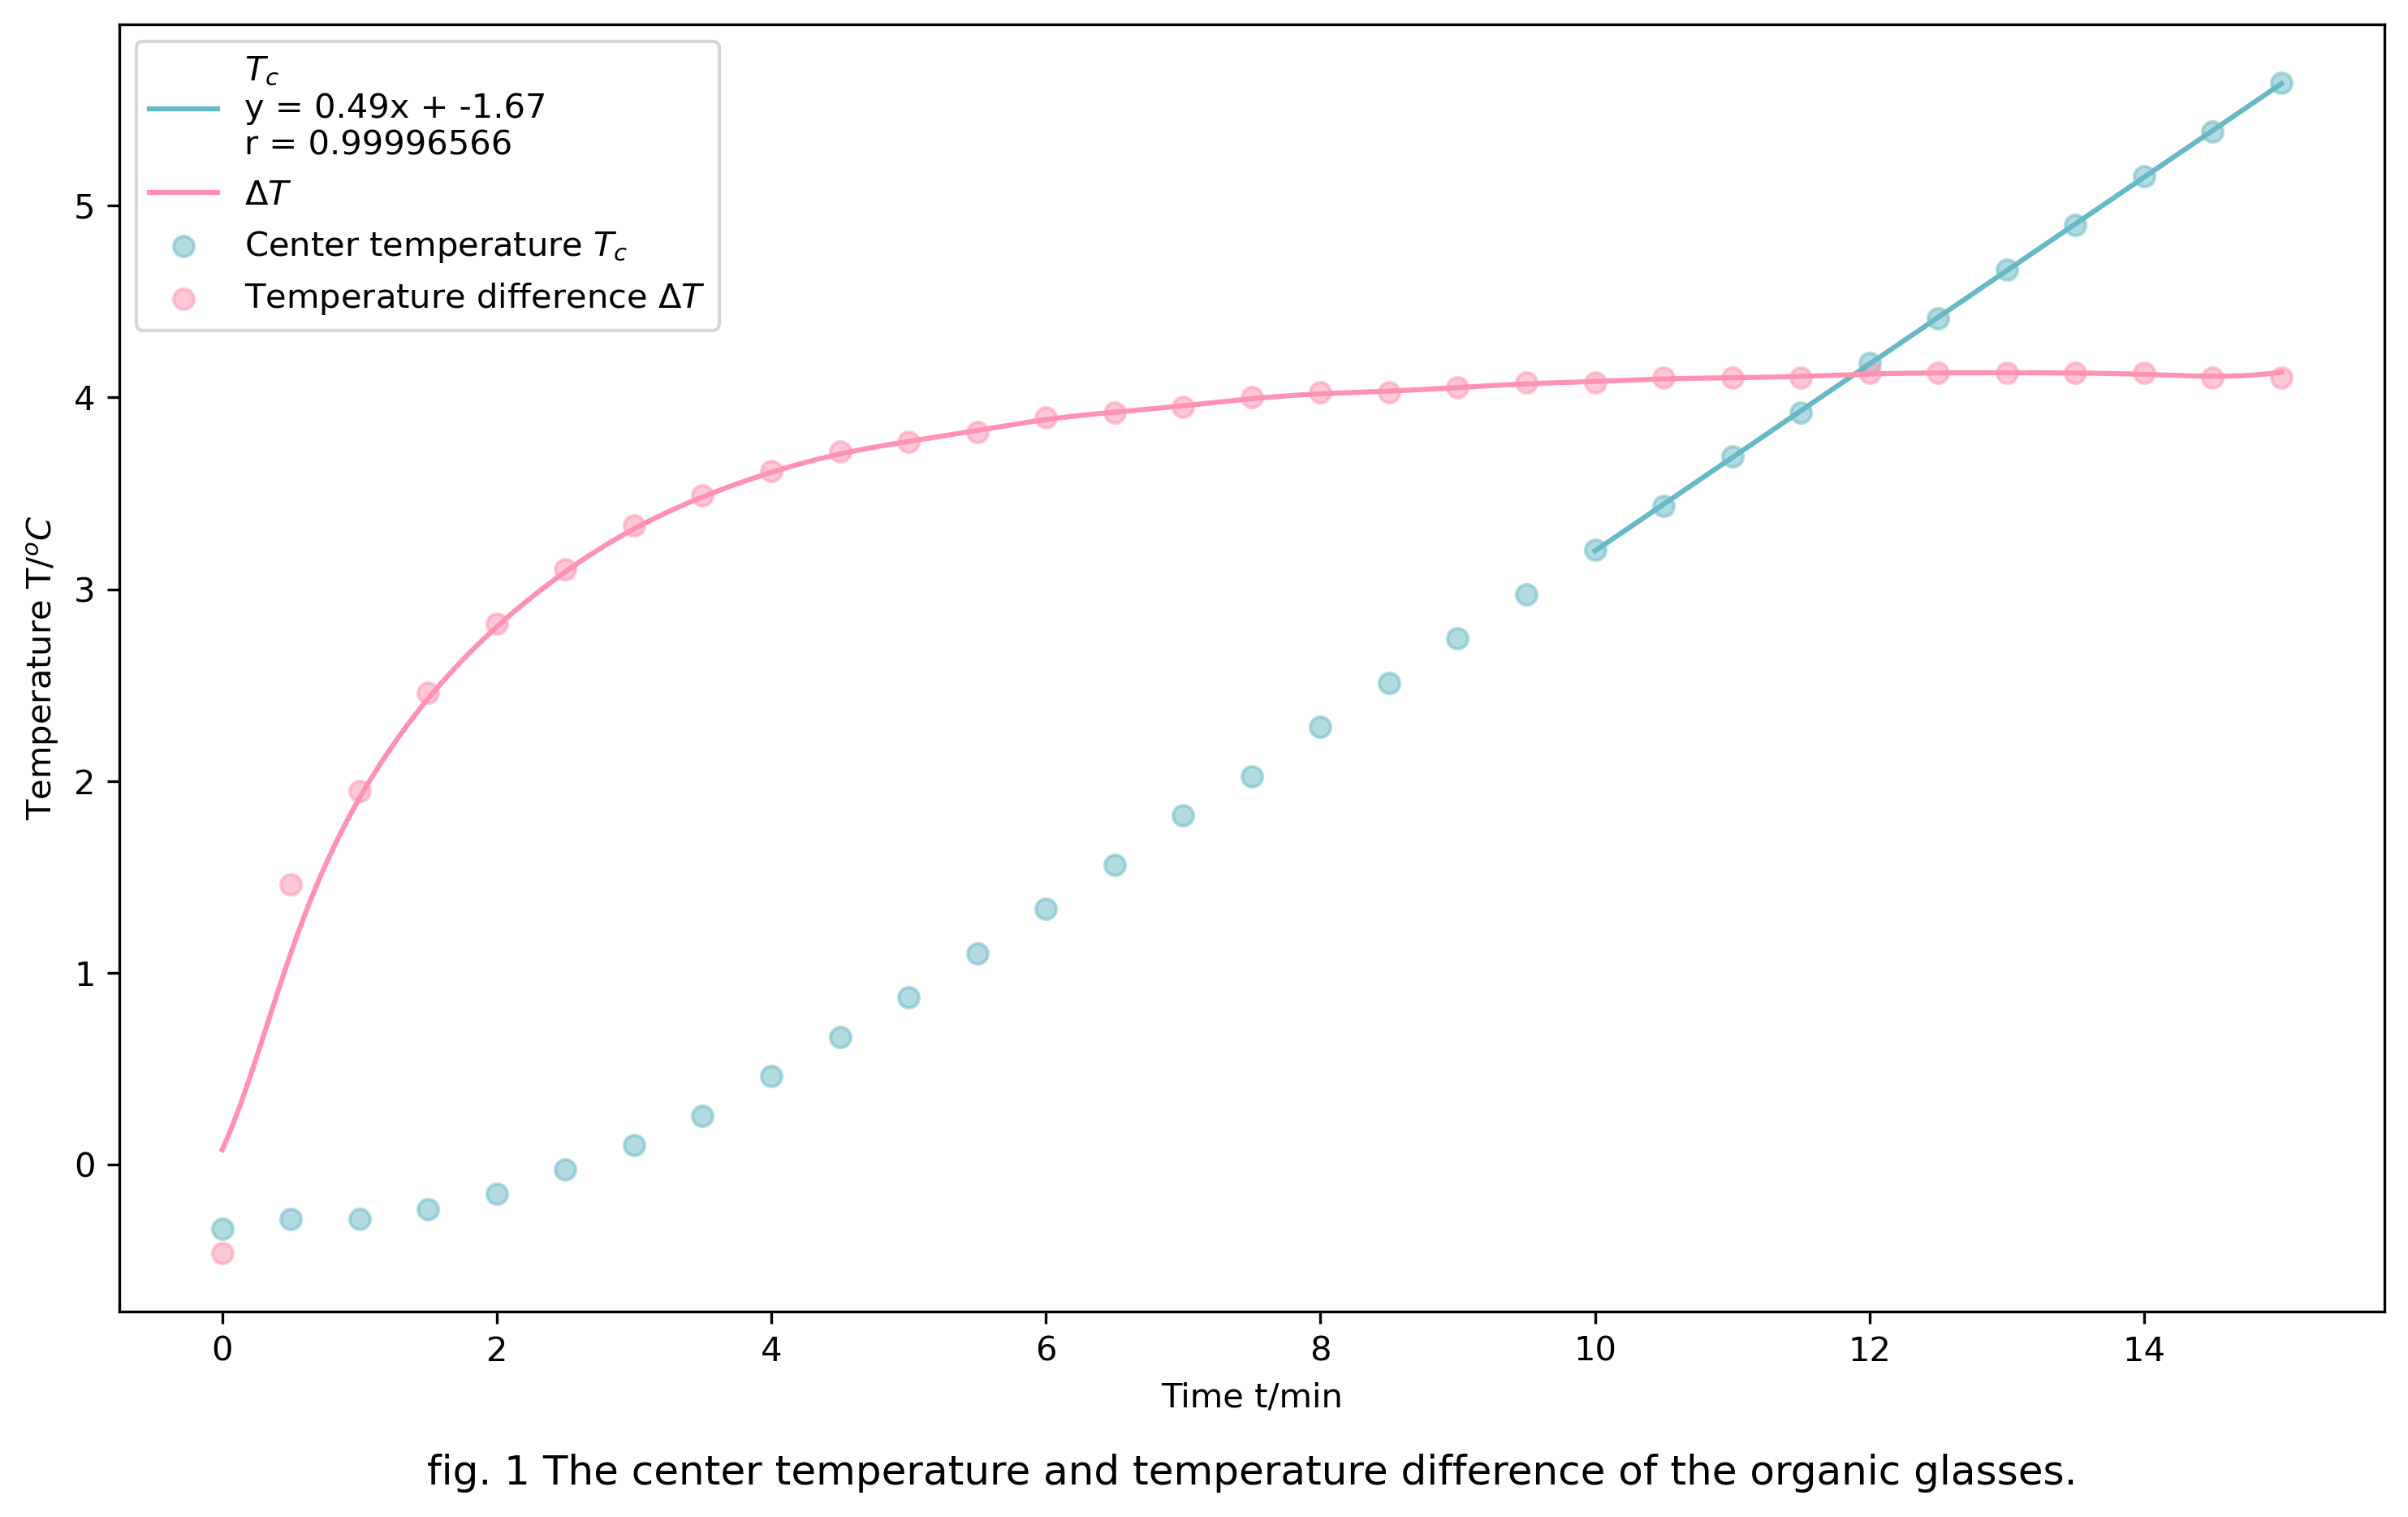
\includegraphics[width=0.4\textwidth]{attachments/fig.1.png}
		\caption{有机玻璃升温中心面温度和温差曲线}
		\label{fig:1}
	\end{figure}	

	我们发现,在加热$10min$后,中心面和加热面温差恒等($\Delta t = 4.10 ^oC$),
	中心面温度线性上升(速率$\frac{dt}{d\tau} = 0.49 ^oC/min$)。系统达到准稳定态。

	由式\ref{eq:1.5.1},式\ref{eq:1.5.2},式\ref{eq:2}和式\ref{eq:3},代入实验参数,
	计算导热系数$\lambda$和热容$c$得:
	\begin{align}
		\lambda &= 0.17166 \pm 0.00033 W \cdot m^{-1} \cdot K^{-1} \\
		c &= 1423.5 \pm 2.7 J \cdot kg^{-1} \cdot K^{-1}
	\end{align}

	\subsection{测量橡胶材料导热系数$\lambda$和热容$c$}

	橡胶材料升温曲线如图\ref{fig:2}
	\begin{figure}[htbp]
		\centering
		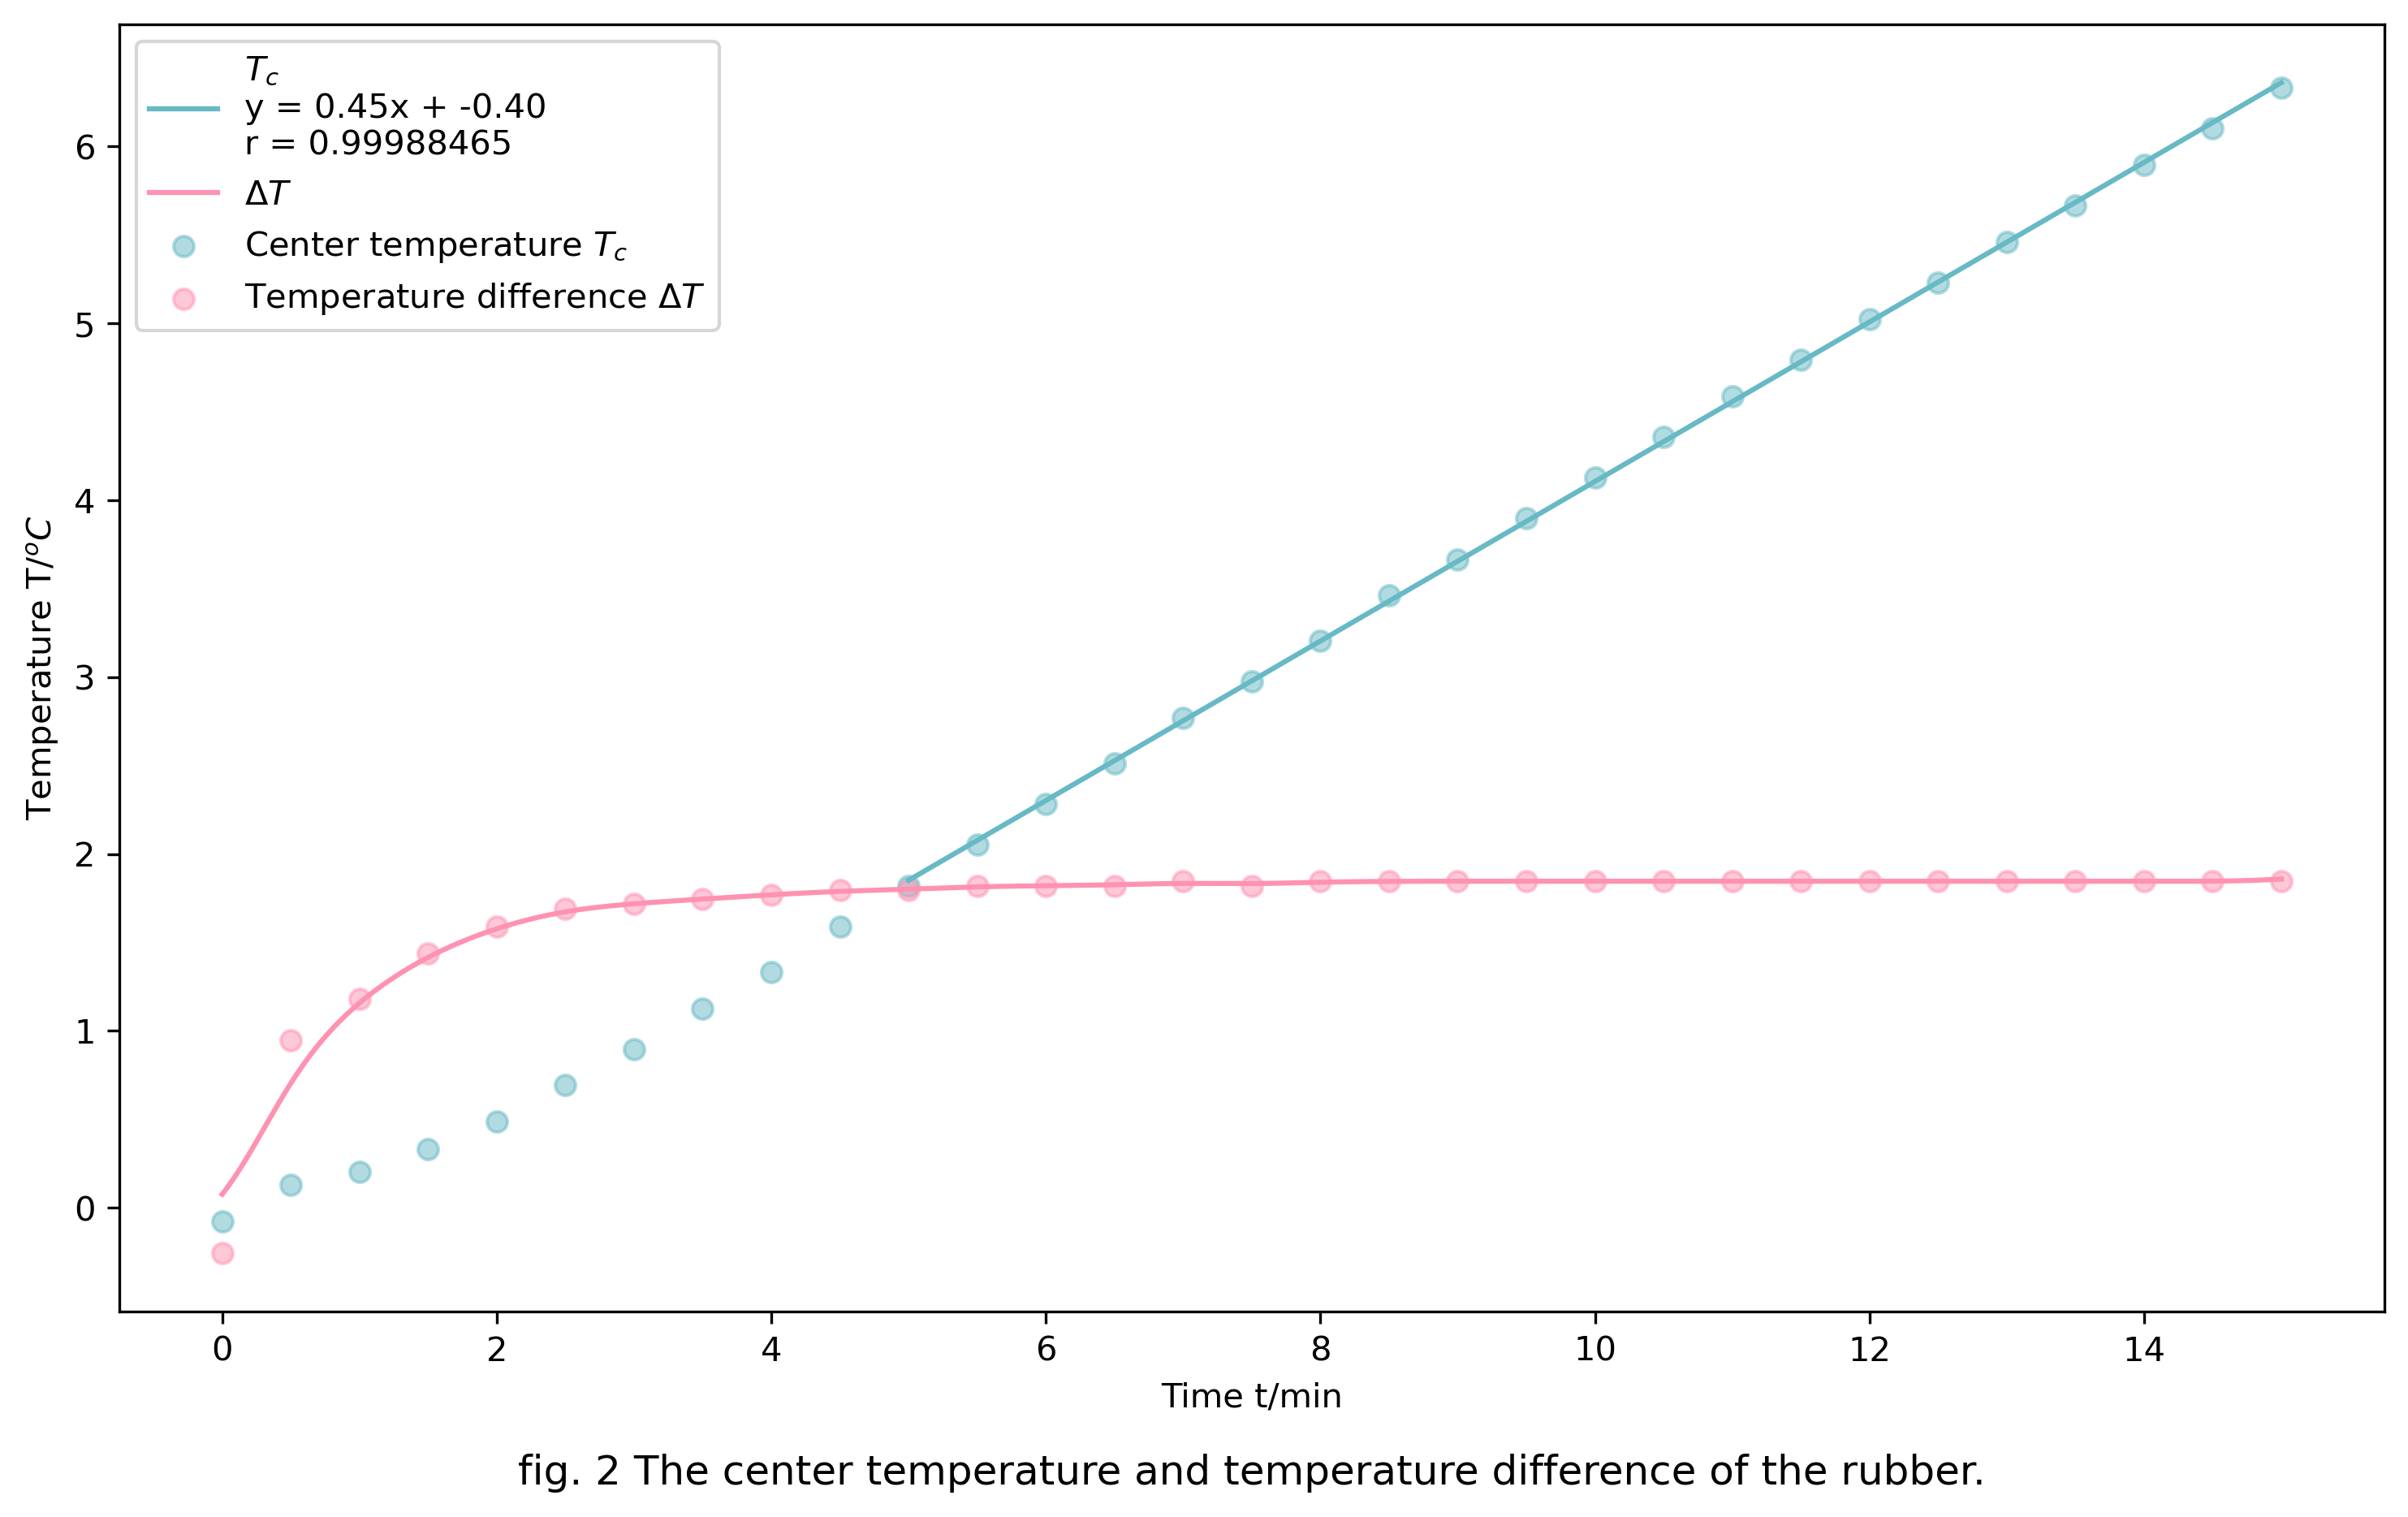
\includegraphics[width=0.4\textwidth]{attachments/fig.2.png}
		\caption{橡胶升温中心面温度和温差曲线}
		\label{fig:2}
	\end{figure}	

	我们发现,在加热$5min$后,中心面和加热面温差恒等($\Delta t = 1.85 ^oC$),
	中心面温度线性上升(速率$\frac{dt}{d\tau} = 0.45 ^oC/min$)。系统达到准稳定态。

	由式\ref{eq:1.5.1},式\ref{eq:1.5.2},式\ref{eq:2}和式\ref{eq:3},代入实验参数,
	计算导热系数$\lambda$和热容$c$得:
	\begin{align}
		\lambda &= 0.38147 \pm 0.00100 W \cdot m^{-1} \cdot K^{-1} \\
		c &= 1349.2 \pm 4.1 J \cdot kg^{-1} \cdot K^{-1}
	\end{align}

\section{讨论}
在本实验中,我们利用准稳态法测量了有机玻璃和橡胶材料的导热系数$\lambda$和热容$c$。
对比我们的实验结果和参考值(有机玻璃零摄氏度下导热系数约$0.2W \cdot m^{-1} \cdot K^{-1}$,热容约$1500 J \cdot kg^{-1} \cdot K^{-1}$;
橡胶材料由于实验用橡胶具体种类不明,无法查阅参考值)发现,有机玻璃测量结果与参考值较为接近,但仍有一定偏差。

分析实验流程,我们认为可能的主要实验误差有:
\begin{enumerate}[label=\arabic*.]
	\item 实验样品材料并非理想无限大导热模型,虽然对面积引入了边缘修正因子$A$,但$A$大小的确定是经验性的,这可能会引入较大误差。
	\item 实验用样品材料尺寸并非绝对一致均匀相同,中心面两侧样品厚度并非完全相等,这可能对导热带来影响。
	\item 实限于实验条件,冷端并非置于摄氏零度环境,但我们参考的热电偶分度表是基于冷端摄氏零度标定的,因此热电偶温度-电压系数可能并不准确。
	\item 橡胶材料具有弹性,使用游标卡尺测量难以控制,这会引入测量误差。
	\item 由于实验须在升温过程中手动记录数据并切换电压测量,难以把握记录时机,可能时间记录并不完全准确。
\end{enumerate}

%%end-------------------正文-----------------------%%

%%end--------------------结论和引用------------------------%%
\section{结~~~论}
在本实验中,我们利用准稳态法测量了有机玻璃和橡胶材料的导热系数$\lambda$和热容$c$,
发现两者的导热系数都较低,有机玻璃导热系数比橡胶小;
而有机玻璃热容比橡胶大。

我们发现使用准稳态法可以方便的测量不良导体的导热系数和热容,但仍存在一定的实验误差,有更进一步的改进的空间。

\printbibliography[title=参考文献] 
%%end--------------------结论和引用------------------------%%


%%begin------------------英文摘要------------------------%%
\twocolumn[
\begin{@twocolumnfalse}
	\renewcommand{\abstractname} {} 
	\begin{center}
	    {\LARGE\bfseries Measurement of thermal conductivity of bad conductors by quasi-steady state method \footnotemark[1]  \par}
	    \vskip 1.4em
	    {\large
	     \lineskip .75em
	      \begin{tabular}[t]{c}
	        \large Ziwei, Huang$^{1}$
	      \end{tabular}\footnotemark[2] \par
	      }
	      \vskip 0.4em
	    {\normalsize 1 Zhongshan School of Medicine, Sun Yat-sen University, Guangzhou  { \rm 510275}, China}
	\end{center}
	\begin{abstract}
		\vspace{-2em}  
	    	{\bf Abstract:}
	     {\small Heat conduction is one of the three forms of thermal transmission, and the heat conduction of thermal conductors follows the heat conduction equation. 
         Thermal conductivity and specific heat are two important parameters in describing the heat-conducting capabilities of heat conductors. 
         In this experiment, we measured the thermal conductivity and specific heat of Plexiglas and rubber materials based on thermocouple temperature measurement and quasi-steady-state method, 
         aiming to investigate the thermal conductivity law of poor conductors. 
         The specific heat of the plexiglass material is $1423.5 \pm 2.7 J \cdot kg^{-1} \cdot  ^{\circ}C^{-1}$ and the thermal conductivity is $\lambda = 0.17166 \pm 0.00033 W \cdot m^{-1} \cdot K^{-1}$; 
         the specific heat of the rubber is $1349.2 \pm 4.1 J \cdot kg^{-1} \cdot  ^{\circ}C^{-1}$ and the thermal conductivity is $\lambda = 0.38147 \pm 0.00100 W \cdot m^{-1} \cdot K^{-1}$}.
	  	\par
		\textbf{Key words}:Quasi-steady-state method, poor conductor, thermocouple, specific heat, thermal conductivity
	\end{abstract}
\end{@twocolumnfalse}
]
\footnotetext[1]{{Supported and taught by Luyoutang, School of Physics, Sun Yat-sen University}}
\footnotetext[2]{{Corresponding author. \url{huangzw29@mail2.sysu.edu.cn}}}
%%end--------------------英文摘要------------------------%%
\end{document}